
\documentclass[11pt]{article}
\usepackage[margin=1in]{geometry}
\usepackage{amsmath,amssymb,siunitx,graphicx,booktabs,tabularx,array,makecell,hyperref,caption,subcaption,float,enumitem,url}
\sisetup{separate-uncertainty=true}

\title{Cavendish Torsion Balance Measurement of the Gravitational Constant}
\author{\textbf{Hongyu Wang}\\Partner(s): Cici Zhang}
\date{\today}

\begin{document}
\maketitle

\section*{Abstract}
We measured the gravitational constant $G$ using a PASCO AP-8215A Cavendish torsion balance and an optical-lever readout.
All three PASCO analysis methods were treated quantitatively.
Method II (equilibrium centers from damped oscillations) applied to three long datasets yielded equilibrium shifts $\Delta S=5.908$--13.427\,cm and corrected values
$G_0=(1.53$--$3.48)\times10^{-10}\,\si{N\,m^2\,kg^{-2}}$.
Method III (early-time acceleration) gave $G_0=(3.94\pm0.08)\times10^{-10}\,\si{N\,m^2\,kg^{-2}}$.
Method I (final deflection) could not be executed as prescribed: even after leaving the apparatus undisturbed overnight ($\sim$1 day), the spot continued to oscillate and drift, so resting endpoints $S_1,S_2$ were not observable.
We therefore report a \emph{Method-I simulation} using the run with the largest excursions, defining ``endpoints'' by robust distribution envelopes (1\%--99\% quantiles), yielding $\Delta S_{\mathrm{M1,sim}}\approx 60.7$\,cm (not a valid $G$ measurement, but a stress test).
To move beyond qualitative discussion, we convert key environmental/mechanical effects into an equivalent spurious $\delta(\Delta S)$ and thus a fractional bias $\delta G/G$.

\section{Introduction}
A Cavendish torsion balance measures extremely small horizontal gravitational forces.
Using accepted $G$ and our geometry (Table~\ref{tab:params}), the expected near-force scale is
\begin{equation}
F_{\mathrm{sig}} \equiv G\frac{m_1 m_2}{b^2} \approx 2.15e-09\ \si{N},
\end{equation}
consistent with the PASCO manual's $\sim 10^{-9}$\,N scale.
Because the signal is so small, modest environmental changes (people moving, carts rolling, doors opening) and subtle mechanical effects (table sag, ribbon creep) can generate comparable torques and bias the measured deflection.
PASCO provides three analysis methods:
Method I (final deflection), Method II (equilibrium centers from damped oscillations), and Method III (acceleration).

\section{Theory and explicit formulas}
\subsection*{Optical lever}
Switching the source masses reverses the equilibrium twist from $-\theta$ to $+\theta$.
The reflected beam changes direction by $4\theta$, giving
\begin{equation}
\theta = \frac{\Delta S}{4L},\qquad \Delta S\equiv S_2-S_1 .
\label{eq:theta}
\end{equation}

\subsection*{Method I/II: deflection equation (PASCO)}
PASCO derives
\begin{equation}
G=\frac{\pi^2 \Delta S\, b^2}{m_1 L d}\,
\frac{\left(d^2+\frac{2}{5}r^2\right)}{T^2},
\label{eq:pasco_deflection}
\end{equation}
and applies the far-mass correction
\begin{equation}
\beta=\frac{b^3}{\left(b^2+4d^2\right)^{3/2}},\qquad 
G_0=\frac{G}{1-\beta}.
\label{eq:beta}
\end{equation}

\subsection*{Method III: acceleration equation (PASCO)}
From the initial acceleration $a_0$,
\begin{equation}
G=\frac{b^2 a_0}{2m_1},\qquad
a_0=\left(\frac{\Delta S}{t^2}\right)\frac{d}{L},
\label{eq:method3}
\end{equation}
where $\Delta S(t)=S(t)-S_1$ and the slope $k\equiv \Delta S/t^2$ over the first $\sim$60\,s is used.

\subsection*{Expected deflection scale (sanity check)}
If the accepted value $G_{\mathrm{true}}=\SI{6.674e-11}{N\,m^2\,kg^{-2}}$ is inserted into Eq.~\eqref{eq:pasco_deflection}, the expected spot shift is
\begin{equation}
\Delta S_{\mathrm{exp}} = \frac{G_{\mathrm{true}}(1-\beta)m_1 L d}{\pi^2 b^2}\,
\frac{T^2}{\left(d^2+\frac{2}{5}r^2\right)}\approx \SI{2.57}{cm}.
\label{eq:deltaS_expected}
\end{equation}
This benchmark is useful when judging whether observed $\Delta S$ is plausible or is being contaminated by non-gravitational effects.

\section{Methods}
\subsection{Apparatus and alignment}

We used a PASCO AP-8215A torsion balance with two $\SI{1.5}{kg}$ source masses and a torsion pendulum carrying two $\SI{38.3}{g}$ test masses.
The optical readout was an optical lever: a laser beam reflects from the pendulum mirror to a distant scale, so small mirror rotations map to measurable spot shifts.

\paragraph*{Leveling (manual leveling sight).}
Following the PASCO procedure, the base was leveled using the three leveling feet while viewing through the built-in leveling sight.
Our primary criterion was that the reflection of the pendulum bob in the mirror appeared centered in the sight aperture.
In practice this step was extremely sensitive: sub-turn changes in a single leveling foot produced visibly different ``top/bottom'' gap symmetry, so the leveling was iterated many times.

\paragraph*{Vertical clearance and plate contact checks.}
The manual notes that the pendulum bob height must be adjusted so the bob is flush with the chamber floor and the pendulum moves freely without contacting the case plates.
During setup we repeatedly verified clearance by observing the small spheres relative to the front/back plates while the system oscillated.
Despite these checks, later inspection of the time series revealed intermittent high-frequency bursts and a shortened apparent period, consistent with occasional contact between a small sphere (or arm) and a plate.
Such collisions introduce additional non-gravitational restoring forces and invalidate the ideal torsion-oscillator model; we therefore treat this as a dominant potential systematic (Sec.~\ref{sec:sys_period}) and, where possible, excluded obvious collision segments from equilibrium fits.

\paragraph*{Rotational zeroing using window and mirror reflections.}
We mounted the scale on the wall and aligned the case rotation using the beam reflected from the front glass window (reference spot), then aligned the pendulum arm using the mirror-reflected spot.
As in the manual, the goal is that the equilibrium line of the mirror spot is vertically aligned below the window spot.
Fine adjustment was performed with the ``zero adjust'' mechanism, and the thumbscrew was tightened only after alignment was stable.

\paragraph*{Troubleshooting history and operational equilibrium criterion (lab notes).}
Even after following the manual, the system often failed to settle and the apparent equilibrium drifted; across multiple sessions we spent $\sim$10 hours iterating leveling, zeroing, and damping strategies.
To isolate the mechanical ``zero'' without gravitational bias, we temporarily removed the large source masses and adjusted the apparatus until the mirror-reflected red spot oscillated with approximately equal left/right turning amplitudes about a stable midpoint on the scale.
Once this symmetry criterion was met (no-source-mass configuration), we installed the large masses and began long recordings for Methods II/III.

\paragraph*{Source-mass positioning asymmetry ($\delta b$).}
The manual instructs that, when moved to Position I/II, the large spheres should be \emph{just touching} the mechanical stop.
During our alignment we observed that when one source mass appeared fully seated (in contact with the plate/stop), the opposite mass retained a gap of order $\sim\SI{2}{mm}$.
We estimated this gap using a paper-stack gauge (calibrated with a digital caliper), then propagated its effect as an additional geometry uncertainty (Sec.~\ref{sec:sys_b}).


\subsection{Setup diagram (overlap fixed)}
Figure~\ref{fig:setup} separates the geometry into (a) a top view (defining $b,d$) and (b) a side view (defining $L,\Delta S$). Labels were positioned to avoid overlap.

\begin{figure}[H]
\centering
\begin{subfigure}{0.92\linewidth}
\centering
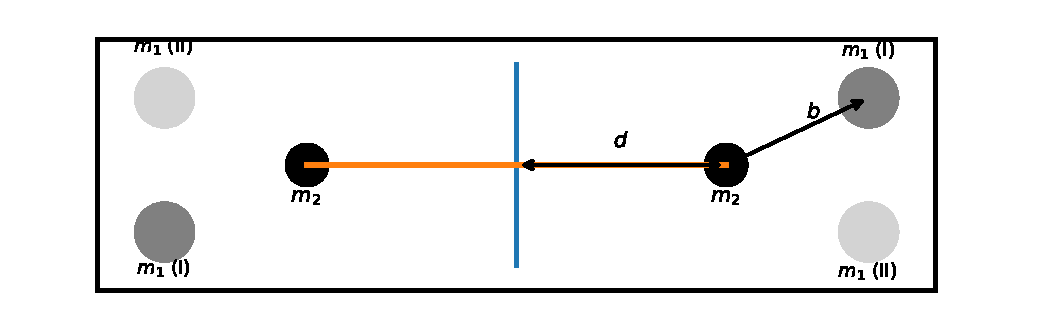
\includegraphics[width=\linewidth]{setup_panel_a.pdf}
\caption{Top view: lever arm $d$, separation $b$, and source-mass positions.}
\end{subfigure}

\vspace{6pt}

\begin{subfigure}{0.92\linewidth}
\centering
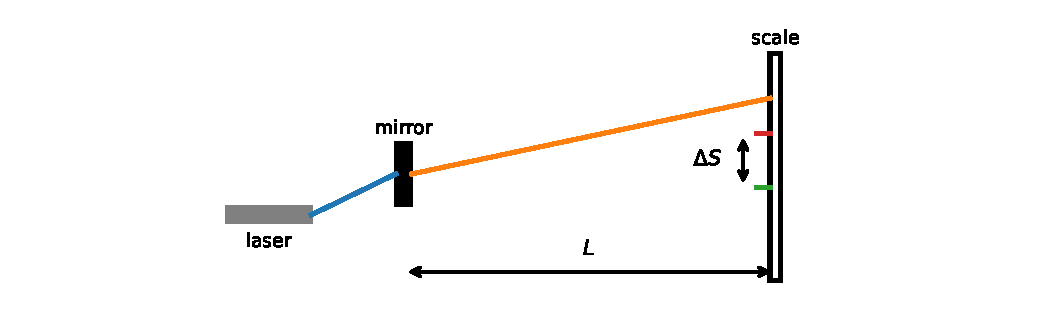
\includegraphics[width=\linewidth]{setup_panel_b.pdf}
\caption{Side view: optical lever. Mirror rotation maps to spot shift $\Delta S$ at distance $L$.}
\end{subfigure}
\caption{Geometry and optical readout used in the analysis.}
\label{fig:setup}
\end{figure}

\subsection{Data acquisition and analysis overview}
Laser-spot motion was recorded by video and tracked with an OpenCV centroid detector (raw CSVs are included in the Overleaf project archive).
For Method II, each long run was split into before/after windows around the mass-swap time and fit to a damped oscillation model to extract equilibrium centers $S_1,S_2$ and the period $T$.
Method I was attempted by leaving the apparatus undisturbed overnight, but the spot never reached a stationary endpoint (quantified below), motivating the simulation approach.

\subsection{Numerical parameters}
Table~\ref{tab:params} lists the values used in calculations.

\begin{table}[H]
\centering
\caption{Parameters used in the analysis.}
\label{tab:params}
\begin{tabular}{@{}lll@{}}
\toprule
Symbol & Meaning & Value \\ \midrule
$m_1$ & source mass (each) & \SI{1.500\pm0.010}{kg} \\
$m_2$ & test mass (each) & \SI{38.3}{g} (nominal) \\
$d$ & lever arm to test mass & \SI{0.0500}{m} \\
$r$ & test mass radius & \SI{0.00819}{m} \\
$b$ & center separation & \SI{0.0422\pm0.0006}{m} \\
$L$ & mirror-to-scale distance & \SI{2.838\pm0.010}{m} \\
$T$ & oscillation period & \SI{292.3\pm12.8}{s} \\
$\beta$ & far-mass factor & 0.0588 \\ \bottomrule
\end{tabular}
\end{table}

\section{Results: numerical values for Methods I--III}
\subsection{Method II (equilibrium centers, three runs)}
Using Method II fits, the equilibrium shifts were
$\Delta S_{\mathrm{YT}}=5.908$\,cm,
$\Delta S_{\mathrm{alt}}=10.618$\,cm,
$\Delta S_{\mathrm{main}}=13.427$\,cm.
Applying Eqs.~\eqref{eq:pasco_deflection}--\eqref{eq:beta} gives the corrected values in Table~\ref{tab:method2}.

\begin{table}[H]
\centering
\caption{Method II results. Quoted uncertainties are \emph{statistical} (propagated from $u_T,u_b,u_L,u_{\Delta S},u_{m_1}$).}
\label{tab:method2}
\begin{tabular}{@{}llll@{}}
\toprule
Run & $\Delta S$ (cm) & $G_0$ ($\si{N\,m^2\,kg^{-2}}$) & $\pm u_{\mathrm{stat}}(G_0)$ \\ \midrule
YouTube benchmark & 5.908 & 1.53e-10 & 1.53e-11 \\
In-lab (alt/full) & 10.618 & 2.76e-10 & 2.60e-11 \\
In-lab (main/100min) & 13.427 & 3.48e-10 & 3.26e-11 \\
\bottomrule
\end{tabular}
\end{table}


\begin{figure}[H]
\centering
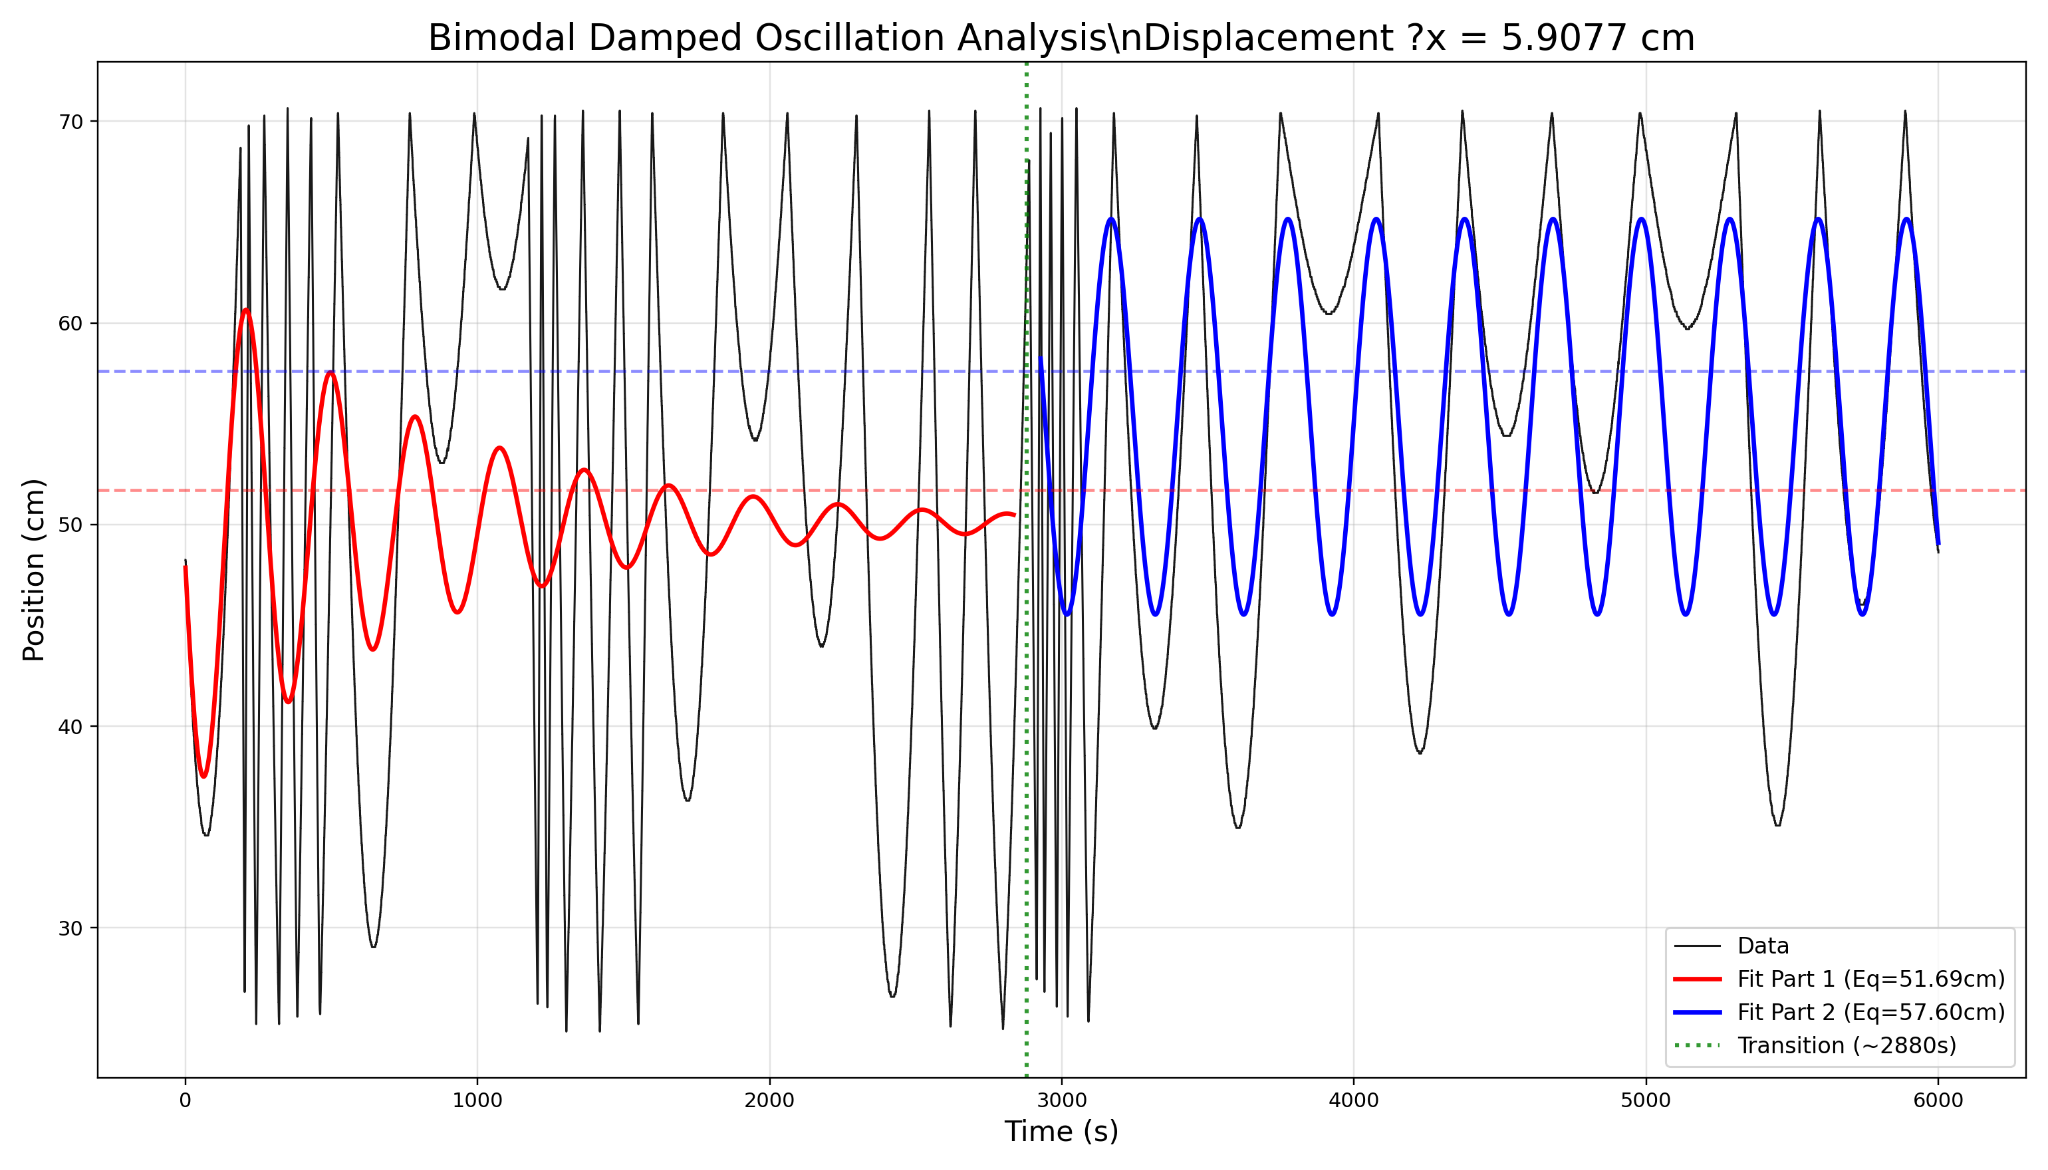
\includegraphics[width=\linewidth]{fit_youtube_100min.png}
\caption{YouTube benchmark run (Method II fit, $\Delta S=5.908$\,cm).}
\label{fig:fit_youtube}
\end{figure}

\begin{figure}[H]
\centering
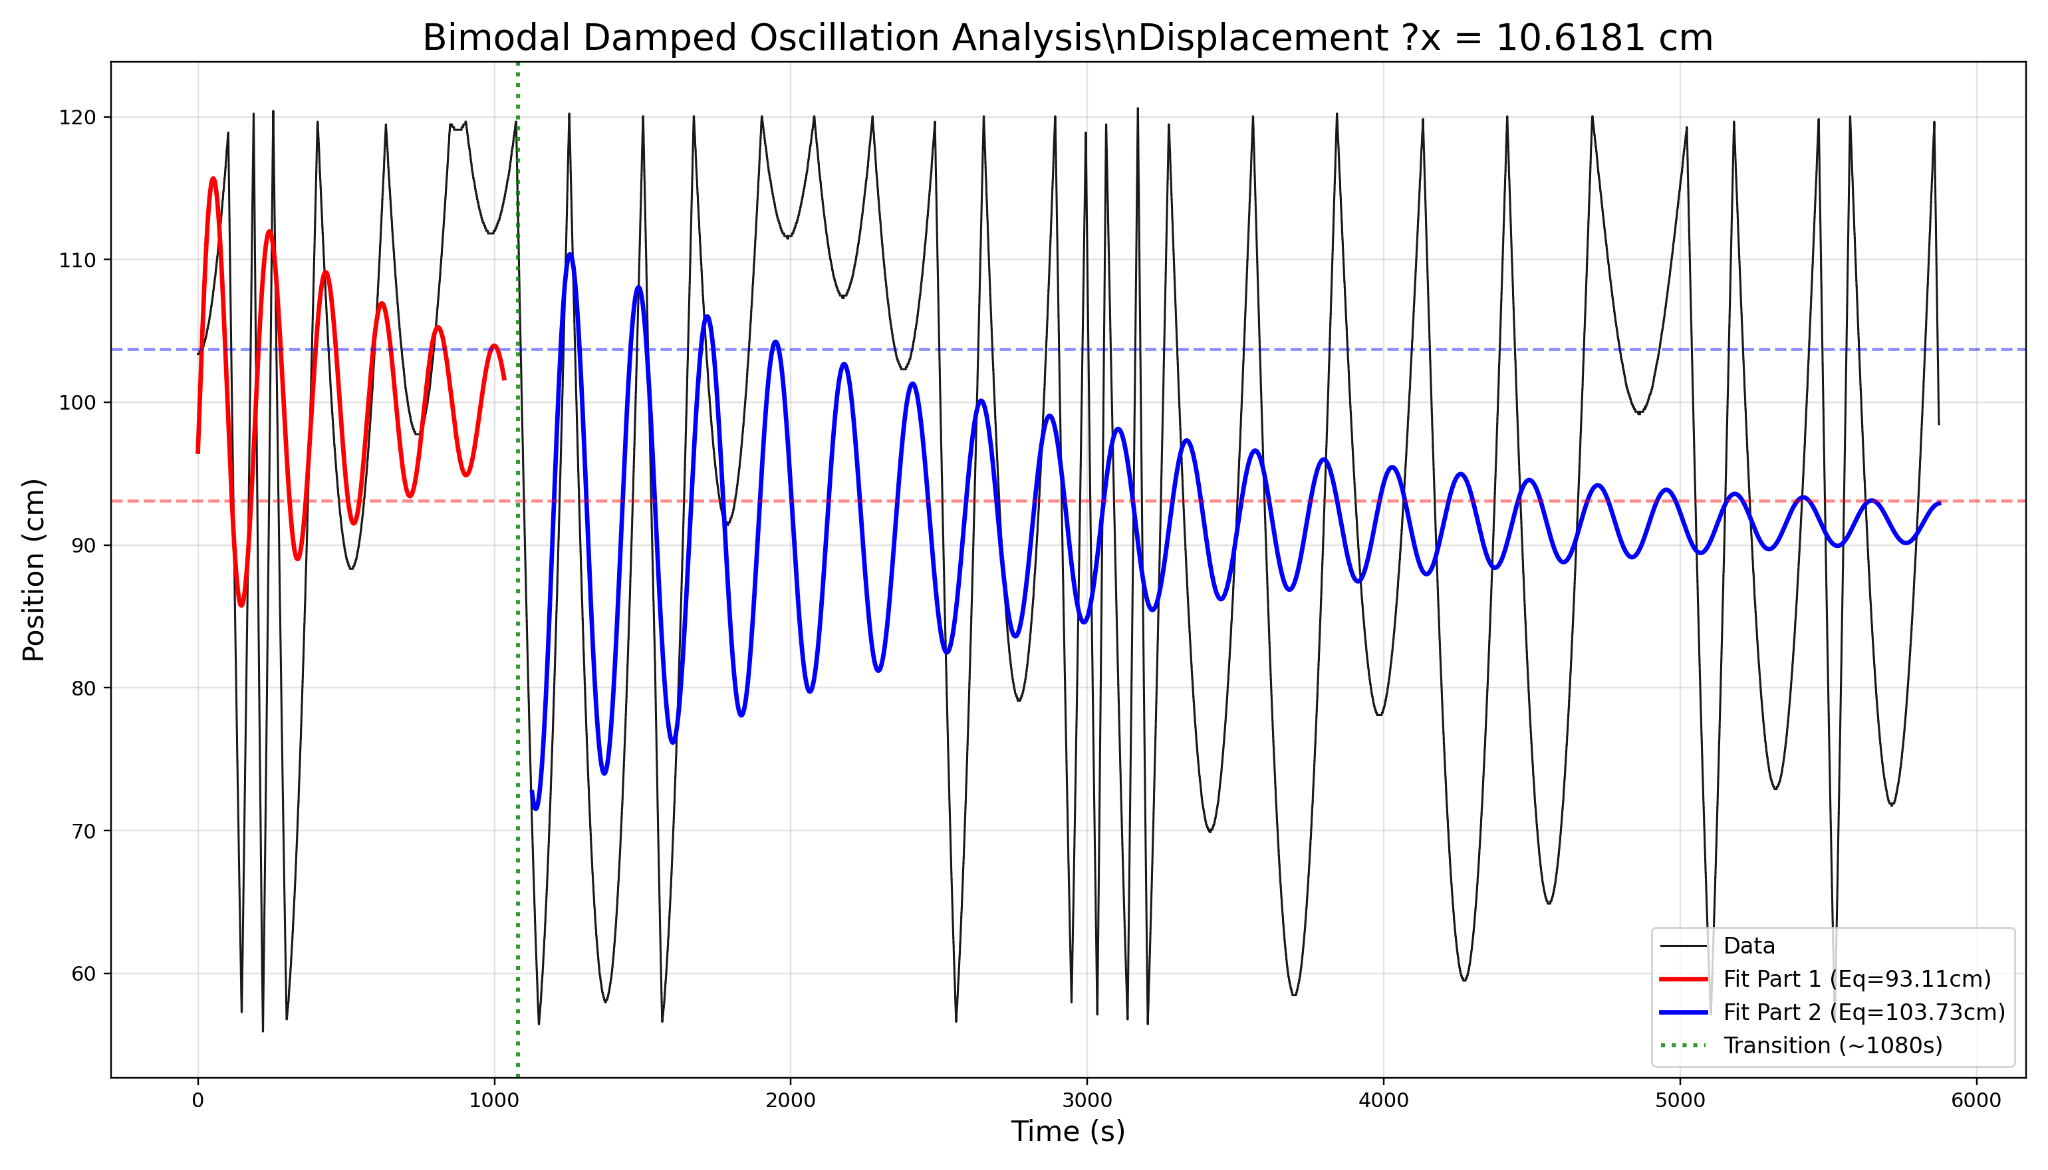
\includegraphics[width=\linewidth]{fit_video_alt_full.png}
\caption{In-lab alt/full run (Method II fit, $\Delta S=10.618$\,cm).}
\label{fig:fit_alt}
\end{figure}

\begin{figure}[H]
\centering
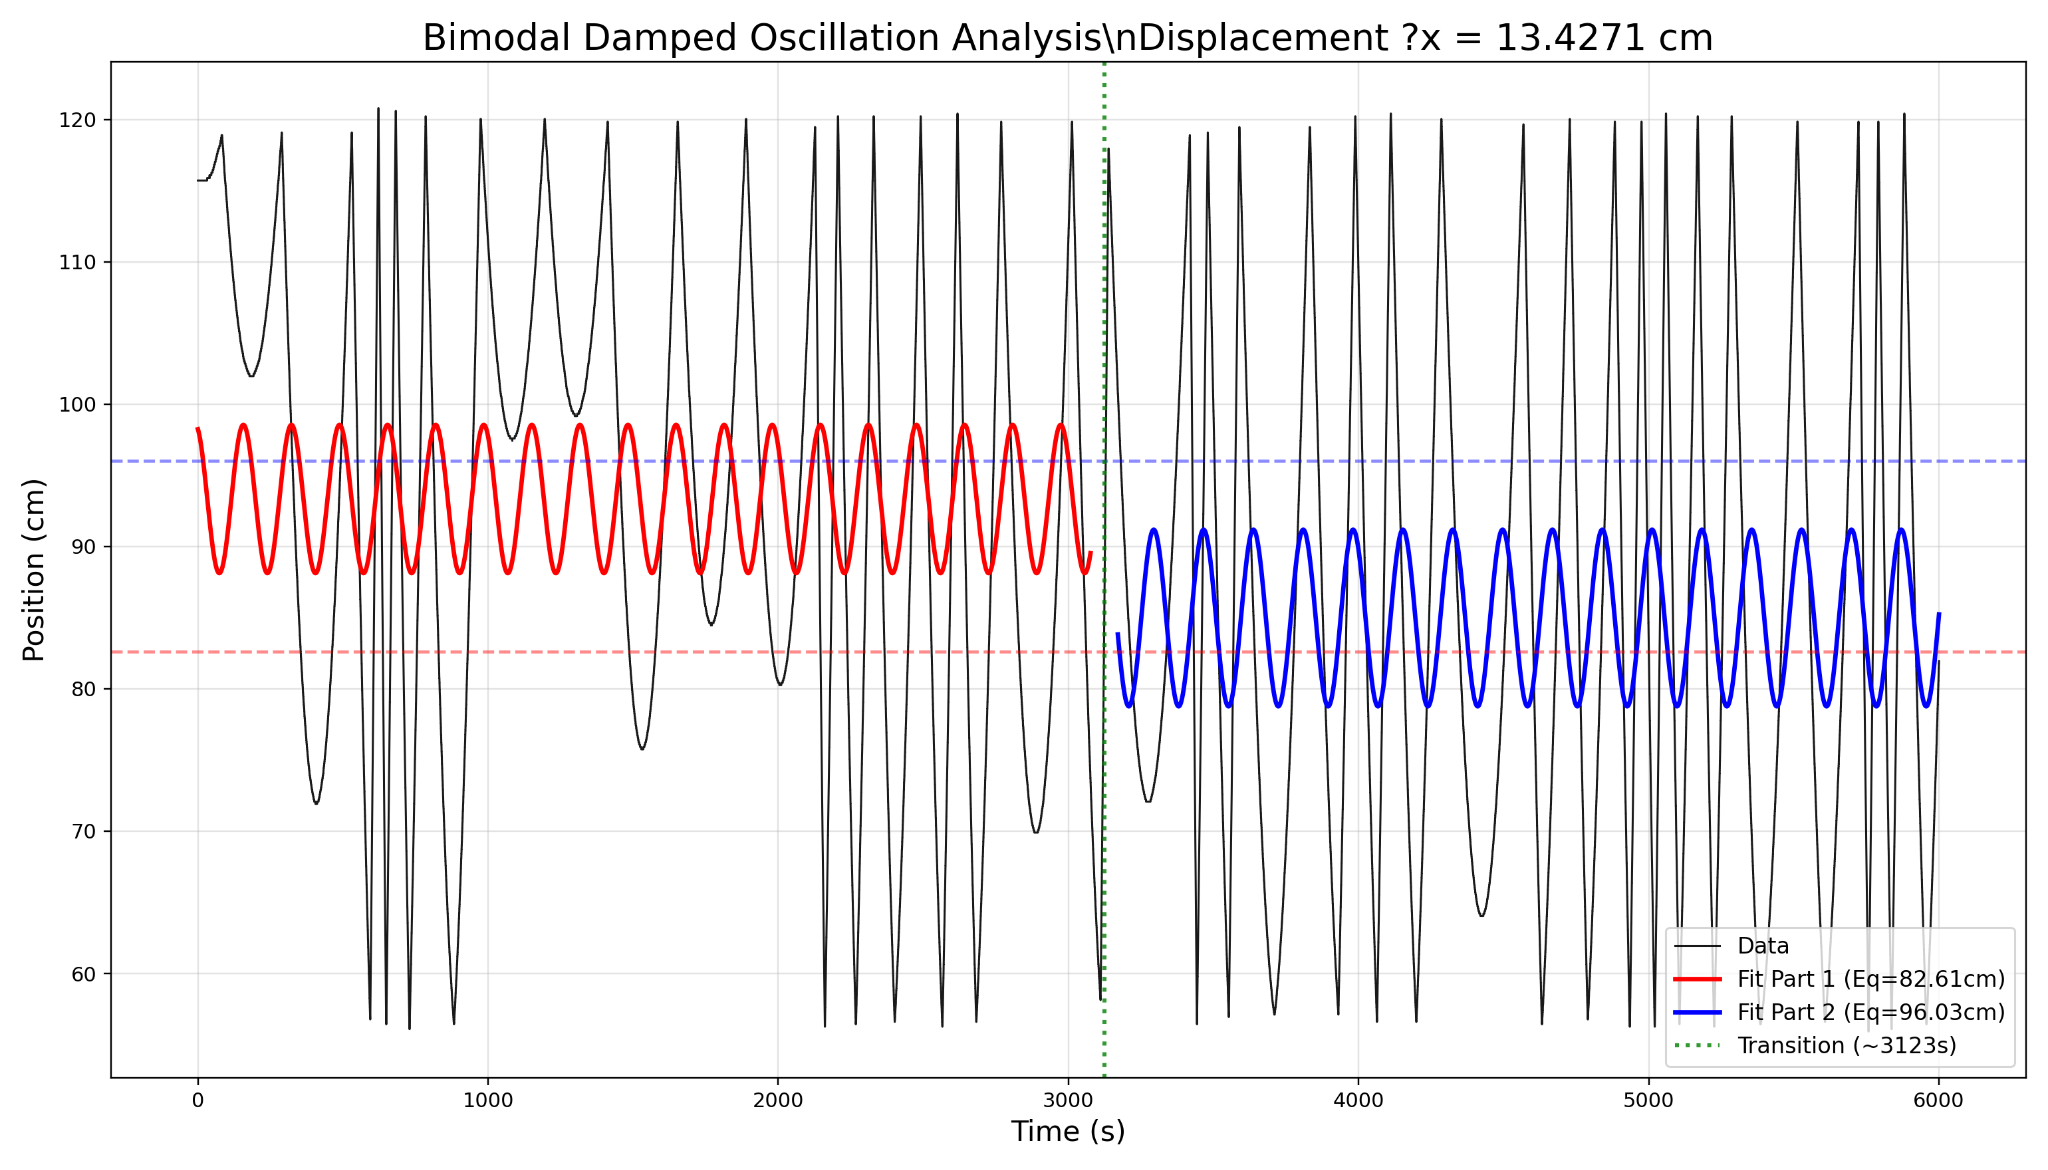
\includegraphics[width=\linewidth]{fit_video_main_100min.png}
\caption{In-lab main/100min run (Method II fit, $\Delta S=13.427$\,cm).}
\label{fig:fit_main}
\end{figure}


\paragraph*{Worked example (Method II, main run).}
With $\Delta S=\SI{13.427}{cm}$, $b=\SI{0.0422}{m}$, $L=\SI{2.838}{m}$, $d=\SI{0.0500}{m}$, $r=\SI{0.00819}{m}$, $m_1=\SI{1.500}{kg}$, and $T=\SI{292.3}{s}$,
\[
d^2+\frac{2}{5}r^2 = 0.002527\ \si{m^2},
\]
\[
G = \frac{\pi^2(0.13427)(0.0422)^2}{(1.500)(2.838)(0.0500)}\frac{0.002527}{(292.3)^2}
= 3.28e-10,
\qquad
G_0=\frac{G}{1-\beta}=3.48e-10.
\]

\subsection{Method III (acceleration)}
From Eq.~\eqref{eq:method3}, the fitted slope $k=\Delta S/t^2$ (0--60\,s) was
\[
k = 0.00355\ \si{cm/s^2},
\qquad
a_0 = k\,(0.01)\frac{d}{L} = 6.25e-07\ \si{m/s^2},
\]
and the worksheet result is
\[
G_0=(3.94\pm0.08)\times10^{-10}\ \si{N\,m^2\,kg^{-2}}.
\]

\subsection{Method I (final deflection) --- why it failed, and a quantitative simulation}
Method I requires \emph{resting} equilibria.
In our lab environment the spot continued to oscillate and drift even after leaving the apparatus undisturbed overnight ($\sim$1 day).
Therefore, unique endpoints $S_1,S_2$ could not be read.
To quantify how badly Method I can fail under these conditions, we simulate ``endpoint'' readings using the \emph{largest-excursion dataset} (main run) and robust envelope quantiles.
For the distributions of $S(t)$ before and after the swap:
\begin{center}
\begin{tabular}{@{}llll@{}}
\toprule
Configuration & $S_{1\%}$ (cm) & $S_{50\%}$ (cm) & $S_{99\%}$ (cm) \\ \midrule
Position I (pre-swap) & 60.97 & 82.61 & 121.19 \\
Position II (post-swap) & 60.97 & 96.03 & 121.70 \\
\bottomrule
\end{tabular}
\end{center}
A naive ``maximum deflection'' endpoint choice gives
\[
\Delta S_{\mathrm{M1,sim}} = S_{99\%}^{(\mathrm{II})}-S_{1\%}^{(\mathrm{I})} \approx 60.7\ \si{cm},
\]
which would imply
\[
G_{0,\mathrm{M1,sim}} \approx 1.58e-09\ \si{N\,m^2\,kg^{-2}},
\]
clearly unphysical. Even moderately less extreme endpoint choices still produce very different answers:
$\Delta S_{10\text{--}90}\approx 52.8$\,cm and
$\Delta S_{5\text{--}95}\approx 57.0$\,cm.
\textbf{Conclusion:} without true settling and drift control, Method I is not merely ``noisy''---it is ill-posed.

\section{Uncertainty propagation (error algorithm) and a concrete budget}
\subsection*{Method I/II statistical uncertainty}
From Eq.~\eqref{eq:pasco_deflection},
\[
\left(\frac{u_G}{G}\right)^2 \approx 
\left(\frac{u_{\Delta S}}{\Delta S}\right)^2
+\left(2\frac{u_b}{b}\right)^2
+\left(\frac{u_L}{L}\right)^2
+\left(2\frac{u_T}{T}\right)^2
+\left(\frac{u_{m_1}}{m_1}\right)^2.
\]
For the main run, the fractional terms are:
\[
\frac{u_{\Delta S}}{\Delta S}=1.67\%,\ 
2\frac{u_b}{b}=2.84\%,\ 
\frac{u_L}{L}=0.35\%,\ 
2\frac{u_T}{T}=8.72\%,\ 
\frac{u_{m_1}}{m_1}=0.67\%,
\]
so $u_{\mathrm{stat}}(G_0)/G_0 \approx 9.36\%$ and $u_{\mathrm{stat}}(G_0)\approx 3.26e-11$.

\subsection*{Quantified systematics as an equivalent $\delta(\Delta S)$}
Table~\ref{tab:sys} converts environmental/mechanical effects into an \emph{equivalent spurious deflection} $\delta(\Delta S)$ using Eq.~\eqref{eq:theta} and the expected signal scale $\Delta S_{\mathrm{exp}}$ from Eq.~\eqref{eq:deltaS_expected}.
Since $G\propto \Delta S$, the corresponding fractional bias is $\delta G/G \approx \delta(\Delta S)/\Delta S$.

\begin{table}[H]
\centering
\small
\setlength{\tabcolsep}{5pt}
\renewcommand{\arraystretch}{1.15}
\caption{Order-of-magnitude systematic effects expressed as equivalent spurious $\delta(\Delta S)$, compared to $\Delta S_{\mathrm{exp}}=\SI{2.57}{cm}$.}
\label{tab:sys}
\begin{tabularx}{\linewidth}{@{}l>{\raggedright\arraybackslash}Xcc@{}}
\toprule
Effect & Model/Formula & $\delta(\Delta S)$ (cm) & $\delta(\Delta S)/\Delta S_{\mathrm{exp}}$ \\ \midrule
70\,kg person at 1\,m & \(F=Gm_2M/r^2\); \(\tau\sim Fd\) & 0.11 & 4.2\% \\
Person moving 1m$\to$2m & \(\Delta F=F(1)-F(2)\) & 0.08 & 3.1\% \\
Base tilt 0.1\,mrad & \(\delta S\approx 4L\delta\theta\) & 0.11 & 4.4\% \\
Base tilt 0.5\,mrad & \(\delta S\approx 4L\delta\theta\) & 0.57 & 22.1\% \\
Ribbon drift (example) & slow drift over hours & 0.50 & 19.4\% \\
Source-mass spacing asymmetry (\(\delta b\approx\SI{2}{mm}\)) &
\makecell[l]{\(f=\tfrac12\!\left[1+\left(\frac{b}{b+\delta b}\right)^2\right]\)\\
\(\delta(\Delta S)\approx(1-f)\Delta S_{\mathrm{exp}}\)} & 0.11 & 4.4\% \\
Finite-twist geometry & \(\delta F/F\approx 2(d\theta)/b\) & 0.01 & 0.5\% \\
Scale calibration (example) & \(\delta(\Delta S)/\Delta S \sim \delta s/s\) & 0.01 & 0.4\% \\
\bottomrule
\end{tabularx}
\end{table}

\subsubsection*{Source-mass spacing asymmetry ($\delta b$)}\label{sec:sys_b}
The deflection derivation assumes both near separations equal to a single $b$, giving a torque coefficient $2/b^2$.
If the two separations differ (e.g.\ $b_1=b$, $b_2=b+\delta b$), the correct coefficient is
\[
\frac{1}{b_1^2}+\frac{1}{b_2^2}=\frac{2}{b^2}\,f,
\qquad
f\equiv \frac{1}{2}\left[1+\left(\frac{b}{b+\delta b}\right)^2\right].
\]
For $\delta b=\SI{2}{mm}$ and $b=\SI{42.2}{mm}$, $f\simeq0.956$.
Thus, if one analyzes the data with a single nominal $b$ and ignores the asymmetry, the inferred $G$ is biased by $\sim$$(1-f)\approx 4.4\%$ (low), and the expected signal is reduced by the same fraction.

\subsubsection*{Period bias from intermittent sphere--plate contact}\label{sec:sys_period}
In Methods I/II, $G\propto 1/T^2$, so a systematic period error produces
\[
\frac{\delta G}{G}\approx -2\frac{\delta T}{T}.
\]
The PASCO manual notes a typical free oscillation period of order \emph{10 minutes}, whereas our extracted period was $T\simeq\SI{292}{s}\approx \SI{4.9}{min}$.
If plate contact or other constraints shorten the apparent period, $G$ is inflated.
As an order-of-magnitude illustration: if the unconstrained period were $T_{\mathrm{free}}\approx\SI{600}{s}$ but we used $T=\SI{292}{s}$, the inferred $G$ would be larger by a factor $(T_{\mathrm{free}}/T)^2\approx 4.2$.
This is comparable to the factor by which our $G_0$ values exceed the accepted constant, making plate contact a plausible \emph{dominant} systematic mechanism in our data.



If we treat the rows above (excluding the ``0.5\,mrad'' stress case) as independent contributions, a representative systematic uncertainty is
\[
u_{\mathrm{sys}}(\Delta S)\approx \sqrt{\sum_i \delta(\Delta S)_i^2} \approx \SI{0.54}{cm},
\qquad
\frac{u_{\mathrm{sys}}(G)}{G}\approx \frac{u_{\mathrm{sys}}(\Delta S)}{\Delta S_{\mathrm{exp}}}\approx 21.1\%.
\]
This is consistent with the observation that run-to-run variation is much larger than the $\sim$10\% statistical budget.

\subsection*{Other potentially important non-gravitational torques (formula-based bounds)}
The following effects were not independently measured in this run, but can be important at the $10^{-9}$\,N scale:
\begin{itemize}[itemsep=3pt]
\item \textbf{Air currents / convection:} for a sphere, $F_{\mathrm{drag}}\sim \tfrac{1}{2}\rho C_d A v^2$. Even $v=\SI{1}{cm/s}$ gives $F_{\mathrm{drag}}\sim 6\times10^{-9}$\,N, comparable to or larger than $F_{\mathrm{sig}}$. A draft shield and thermal equilibration are essential.
\item \textbf{Electrostatics:} if residual charge $Q$ exists, $F_C \sim k Q^2/r^2$. For $Q=\SI{10}{pC}$ at $r=\SI{4}{cm}$, $F_C\sim 6\times10^{-10}$\,N (tens of percent of $F_{\mathrm{sig}}$). Mitigation: grounding, conductive surfaces, and humidity control.
\item \textbf{Tracking/calibration artifacts:} centroid noise of $\sim$1 pixel corresponds to $\sim$0.06\,cm for a 100\,cm/1625\,px scale, which is already $\sim$2\% of $\Delta S_{\mathrm{exp}}$.
\end{itemize}

\section{Discussion: what cancels, what compounds, and how to improve}
\subsection*{Why results are far from accepted $G$}
Eq.~\eqref{eq:deltaS_expected} predicts $\Delta S_{\mathrm{exp}}\approx\SI{2.57}{cm}$, while the measured Method II shifts were 5.9--13.4\,cm.
This factor-of-2--5 excess cannot be explained by the statistical uncertainty budget ($\sim$10\%), implying dominant systematics.
Table~\ref{tab:sys} shows that even small base tilts or slow drifts can be a large fraction of the expected signal.
In addition, because $G\propto 1/T^2$, any systematic \emph{underestimate} of the oscillation period directly inflates $G$.
Our measured period ($T\approx\SI{292}{s}$) is substantially shorter than the manual's typical $\sim$10\,min scale; if this shortening is caused by intermittent sphere--plate contact (as suggested by abrupt high-frequency segments in $S(t)$ and our alignment logs), it can explain an order-unity bias in $G$ (Sec.~\ref{sec:sys_period}).
Therefore, the key limitation is not random noise but environmental/mechanical reproducibility and model validity (free oscillation without contact).

\subsection*{Do corrections cancel? (A/B/C)}
(A) Constant offsets (static gravitational gradients, constant electrostatic bias, constant laser pointing) cancel to first order in $\Delta S=S_2-S_1$.
(B) Some corrections can oppose each other: the manual's far-sphere correction increases $G$ by $\sim 6.2\%$, whereas finite-geometry corrections can reduce $G$ if modeled; accidental partial cancellation is possible but unreliable.
(C) Many real-lab issues compound (drift + moving masses + asymmetric base deformation + mis-measured $b$), so agreement between methods/runs is a stronger validation than any single correction.

\subsection*{Concrete improvement plan (how to actually fix the experiment)} 
To move toward a high-accuracy measurement, the experiment must explicitly control the dominant systematics:
\begin{enumerate}[itemsep=4pt]
\item \textbf{No-walk zone / gravity hygiene:} prohibit people and rolling carts within $\gtrsim\SI{2}{m}$ during data collection; keep doors closed. Gravity cannot be shielded, only controlled.
\item \textbf{Rigid common-base mounting:} mount the laser, scale, and torsion balance on one rigid platform (or an optical table) to suppress relative tilts during mass switching.
\item \textbf{Drift cancellation by symmetry:} perform I$\rightarrow$II$\rightarrow$I sequences and average the two $\Delta S$ values to cancel linear drift and some creep.
\item \textbf{Measure geometry directly:} measure $b$ on both sides (and verify tangential alignment) with calipers/spacing gauges; if asymmetry remains, use a two-distance torque model rather than a single $b$.
\item \textbf{Fit a drift term explicitly:} use $S(t)=S_0+vt+Ae^{-t/\tau}\sin(\omega t+\phi)$ so slow drift is not absorbed into $\Delta S$.
\item \textbf{Method III protocol tightening:} trigger $t=0$ at the instant mass motion ends; require near-zero intercept in the $\Delta S$ vs.\ $t^2$ fit as a sanity check.
\item \textbf{Thermal/airflow control:} close the case, wait for thermal equilibration, and avoid HVAC drafts; measure temperature to correlate with drift.
\end{enumerate}

\section{Conclusion}
We provided numerical values, formulas, and uncertainty algorithms for all three PASCO methods.
Method II across three long datasets yielded $G_0=(1.53$--$3.48)\times10^{-10}$ with $\sim$10\% statistical uncertainty but much larger systematic variation.
Method III gave $G_0=(3.94\pm0.08)\times10^{-10}$ but is timing/baseline sensitive.
Method I could not be executed because the system never reached resting equilibrium even after overnight settling; an envelope-based simulation shows that ``endpoint'' reading can inflate $\Delta S$ by an order of magnitude, producing meaningless $G$.
The dominant shortcomings of the student-lab implementation are environmental gravity perturbations (moving masses), mechanical base deformation during mass switching, and long-time drift/creep of the torsion ribbon.
A publishable $G$ measurement requires (i) strict control of nearby moving masses, (ii) rigid common-base mounting, (iii) drift-canceling measurement sequences, and (iv) direct geometric verification of $b$ and tangential alignment.


Beyond these headline issues, the magnitude of the observed deflections compared with the expected scale (Eq.~\eqref{eq:deltaS_expected}) indicates that unmodeled low-frequency disturbances and/or calibration/geometry biases dominated our measurement.
The large run-to-run spread in $\Delta S$ and $G_0$ shows that reproducibility, rather than statistical noise, is the limiting factor in a typical student-lab environment.

Future work should therefore prioritize \emph{control and diagnosis} over longer averaging: enforce a strict ``gravity hygiene'' zone during acquisition, mount the laser/scale/balance on a rigid common base, and adopt symmetric measurement sequences (I$\rightarrow$II$\rightarrow$I) so drift and creep can be estimated and subtracted rather than absorbed into $\Delta S$.
On the analysis side, fitting an explicit drift term and validating the optical scale calibration (including pixel-to-centimeter uncertainty and any camera perspective effects) would allow a credible systematic uncertainty budget and a more defensible comparison to the accepted value of $G$.

\section*{References}
PASCO Scientific, \emph{Gravitational Torsion Balance AP-8215A: Instruction Manual with Experiment Guide and Teachers' Notes} (012-11032B).

\end{document}
